\documentclass[../../main.tex]{subfiles}

\begin{document}

    
\subsection{Docker}

 \begin{wrapfigure}{r}{0.5\textwidth}
    % \begin{center}
    \centering
        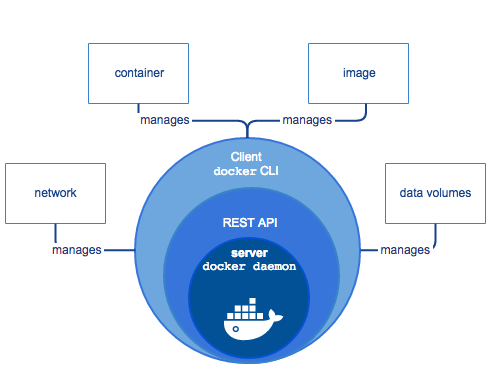
\includegraphics[width=0.45\textwidth]{images/Docker_engine.png}
    % \end{center}
  \caption{Docker Engine technológia\cite{docker_overview}}
%  https://docs.docker.com/engine/images/engine-components-flow.png
\end{wrapfigure}

 Docker je platforma písaná v jazyku GO, ktorá umožňuje spustenie aplikácie vo voľne izolovaných  prostrediach nazývaných kontajnery. Tieto kontajnery nevyžadujú tak veľa zdrojov ako virtuálne stroje bežiace na princípe hypervízora. Rapídne stúpa počet aplikácií, ktoré bežia na tejto platforme. Na jednom hostovskom stroji môže zároveň bežať viac kontajnerov. Docker je vhodný na vývoj, testovanie aj nasadenie aplikácie. Pre budovanie využíva klient-server technológiu Docker Engine, ktorá sa skladá z daemon procesu dockerd, REST API ako rozhranie  inštrukcií a komunikácie medzi programami a Docker Deamon proces a  CLI docker (klient) pomocou ktorého je deamon dockerd ovládaný. Docker kontajner je ľahko prenosný. Je možné jeden kontajner spustiť na vývojárovom počítači, cloude aj virtuálnom stroji.
 \paragraph{Architektúra:}
 Klient komunikuje prostredníctvom REST API, cez UNIX socket alebo sieťové rozhranie s Docker deamon procesom dockerd, ktorý sa stará o budovanie a spúšťanie kontajnera. Dockerd počúva požiadavky Docker API A má na starostí Docker objekty ako sú images, kontajnery, siete a diskové jednotky. Dockerd môže komunikovať aj s ostatnými deamonmi. O hlavnú interakciu sa stará Docker klient, ktorý posiela inštrukcie dockerd deamonu. Využíva pritom Docker API.
 \begin{figure}[h!]
     \centering
     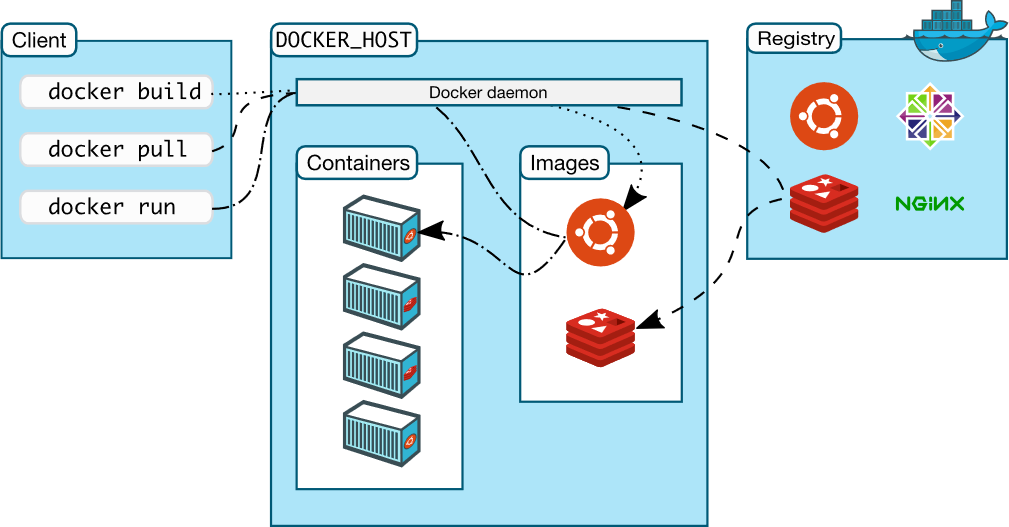
\includegraphics[width =0.9\textwidth]{images/docker_architecture.png}
     \caption{Docker architektúra\cite{docker_overview}}
     \label{fig:docker_architecture}\cite{docker_overview}
 \end{figure}
 \paragraph{Docker objekty}
 \begin{description}
    \item[Images] - vzor pre vytvorenie kontajnera s inštrukciami, väčšinou je založený na iných takýchto obrazoch. Inštrukcie sú uložené v súbore, ktorý sa musí volať Dockerfile, kde každá jedna inštrukcia vytvorí jednu vrstvu kontajnera. Pri zmene súboru a budovaní kontajnera sa vykonávajú len tie inštrukcie, ktoré boli zmenené (defaultne).
    \item[Containers] - spustiteľná inštancia image. Kontajner je možné pripojiť do sietí, pridať mu dátové priestory alebo vytvoriť nový obraz založený na jeho aktuálnom stave. Pri vymazaní kontajnera nie je nič uložené na jeho dátovom priestore. Pri spustení kontajnera sa vyhľadá alebo stiahne image, vytvorí nový kontajner, alokuje sa súborový systém na čítanie a zapisovanie, na vytvorenie alebo zmenu na lokálnom systéme súborov, vytvorí sa sieťové rozhranie s pridelením IP adresy pre kontajner,  naštartuje sa kontajner a spustí sa príkaz, ak bol zadaný Docker klientom.  Pri ukončení kontajner je stopnutý ale nie vymazaný.
    \item[Services] - Umožňuje škálovať kontajneri pomocou viacerých Docker deamonov, ktoré spolupracujú ako jeden roj (swarm). Všetky komunikujú medzi sebou pomocou Docker API. Služba sa javí ako jedna aplikácia.
 \end{description}
 \vspace{1.5cm}
 Pre ukladanie Docker images je vytvorený verejný register takýchto obrazov, ktoré sú dostupné pre užívateľa. Systém je používaním veľmi podobný technológii Github.\cite{docker_overview}
 


% https://www.sciencedirect.com/science/article/pii/S1084804518302273\#sec3
% https://www.pcrevue.sk/a/Kontajnery-ulahcia-virtualizaciu-Linuxu
% https://docs.docker.com/get-started/overview/
% %repositories,containers, images, machine, virtualizacia, LXC (Linux Containers) 


% \subfile{sections/docker/docker_popis.tex}



\begin{figure}[h!]
  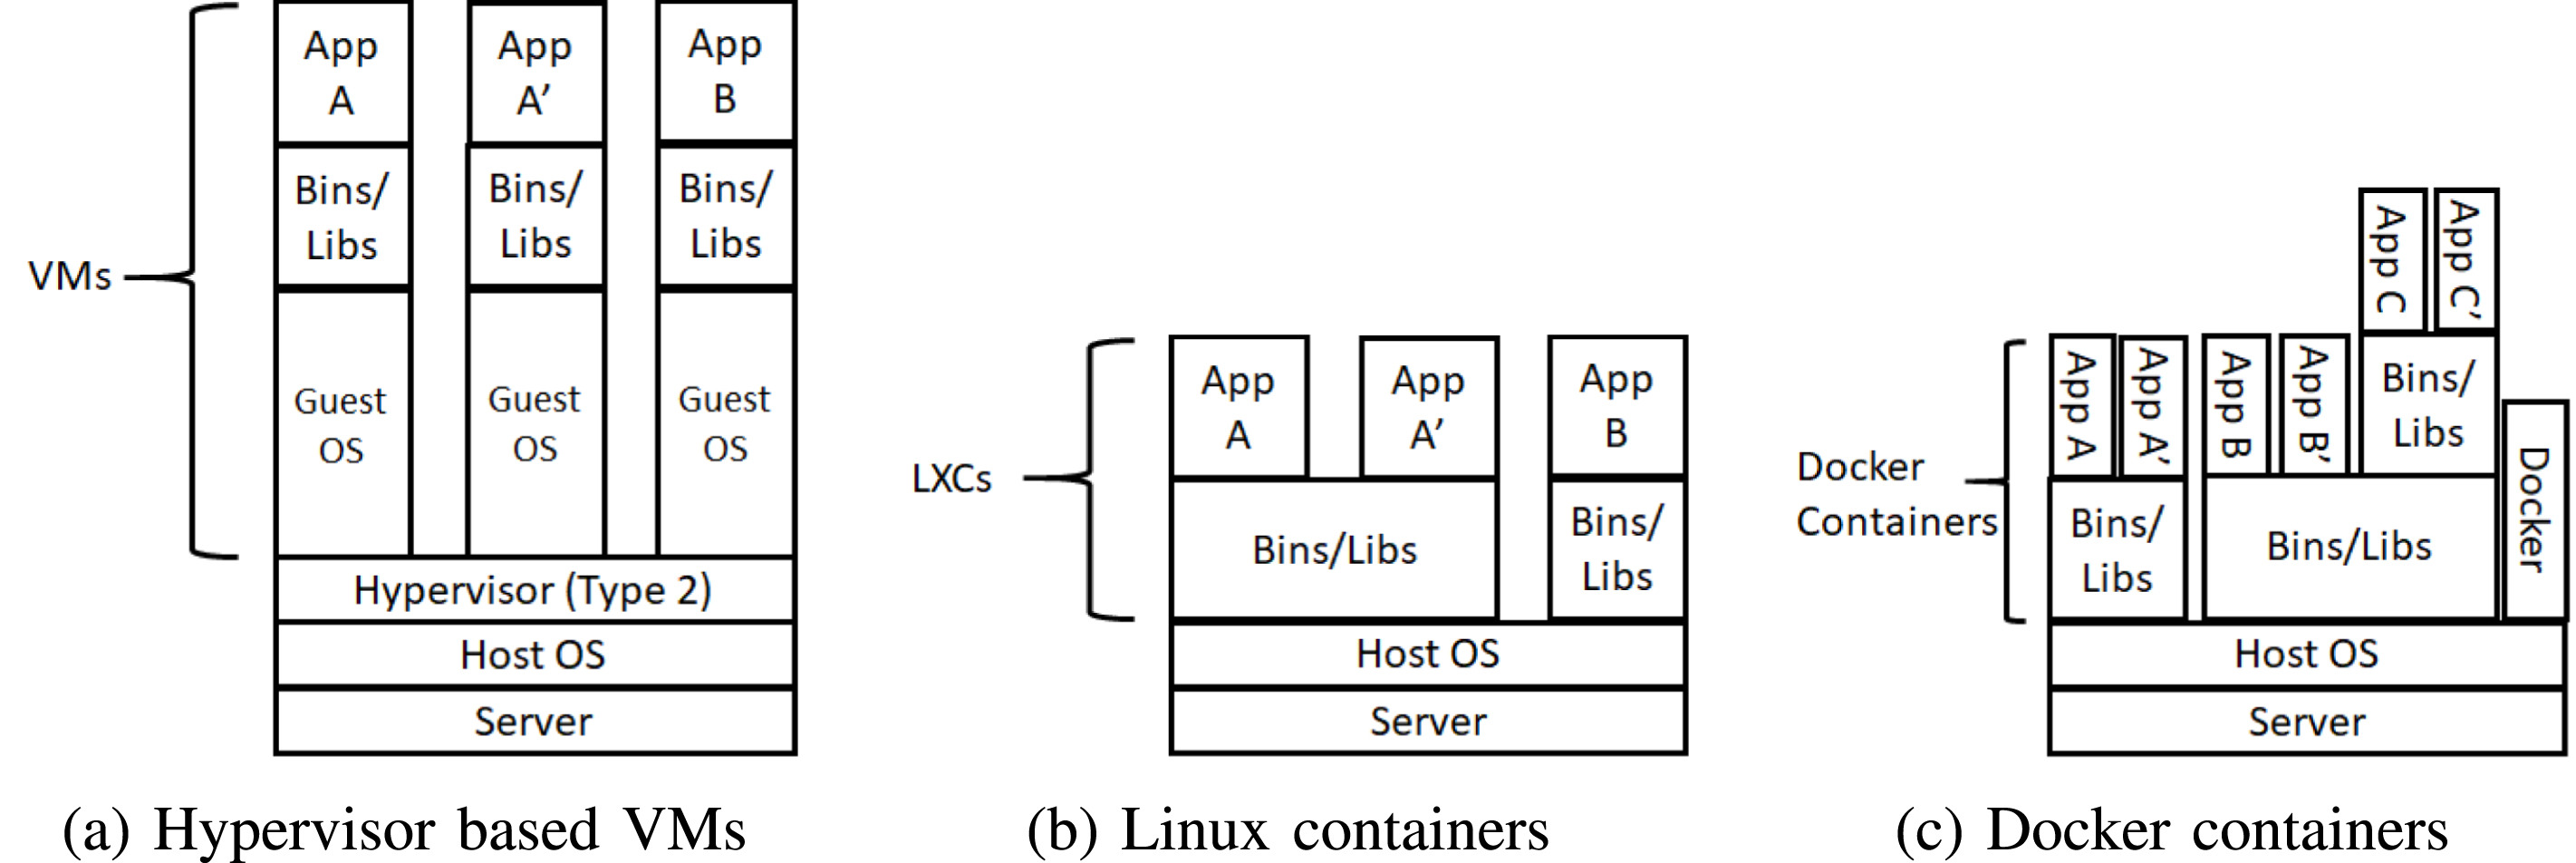
\includegraphics[scale=0.9]{images/containers_vs_LXC.jpg}
  \centering
  \caption{Porovnanie virtualných strojov založených na hypervisore, linuxových kontajnerov a Docker kontajnerov\cite{WAN201897}}
%   https://ars.els-cdn.com/content/image/1-s2.0-S1084804518302273-gr1_lrg.jpg
\end{figure}


\end{document}